\documentclass[10pt]{article}

\usepackage[T1]{fontenc}
\usepackage[utf8]{inputenc}
\usepackage[letterpaper,margin=0.76in,headheight=14pt]{geometry}
\usepackage{microtype}
\usepackage{amsmath,amssymb}
\usepackage{booktabs}
\usepackage{tabularx}
\usepackage{array}
\usepackage{enumitem}
\usepackage{graphicx}
\usepackage{xcolor}
\usepackage{tikz}
\usetikzlibrary{arrows.meta,positioning}
\usepackage{caption}
\usepackage[hidelinks]{hyperref}
\usepackage{fancyhdr}

\definecolor{navy}{HTML}{17324D}
\definecolor{blue}{HTML}{2F6F9F}
\definecolor{lightblue}{HTML}{EAF3F8}
\definecolor{lightgray}{HTML}{F3F5F7}
\definecolor{green}{HTML}{237A57}
\definecolor{orange}{HTML}{B45F06}
\definecolor{textgray}{HTML}{4A5560}

\hypersetup{
  colorlinks=true,
  linkcolor=navy,
  citecolor=navy,
  urlcolor=blue,
  pdftitle={Mini-DLSS: Technical Summary and Evaluation Report},
  pdfsubject={Lightweight temporal video super-resolution},
  pdfkeywords={video super-resolution, temporal reconstruction, ConvGRU, ONNX}
}

\pagestyle{fancy}
\fancyhf{}
\lhead{\small\color{textgray}Mini-DLSS Technical Summary}
\rhead{\small\color{textgray}June 2026}
\cfoot{\small\color{textgray}\thepage}
\renewcommand{\headrulewidth}{0.35pt}

\setlength{\parindent}{0pt}
\setlength{\parskip}{0.55em}
\setlist[itemize]{leftmargin=1.35em,itemsep=0.25em,topsep=0.25em}
\setlist[enumerate]{leftmargin=1.55em,itemsep=0.25em,topsep=0.25em}
\captionsetup{font=small,labelfont=bf}
\renewcommand{\arraystretch}{1.16}

\newcommand{\project}{Mini-DLSS}
\newcommand{\code}[1]{\texttt{#1}}
\newcommand{\metric}[1]{\textbf{\color{navy}#1}}
\newcommand{\sectionrule}{\vspace{-0.45em}\color{blue}\rule{\linewidth}{0.7pt}\color{black}\vspace{0.2em}}
\newcommand{\reportsection}[1]{\section*{\color{navy}#1}\sectionrule\addcontentsline{toc}{section}{#1}}

\newcommand{\callout}[2]{%
  \begin{center}
  \setlength{\fboxsep}{8pt}%
  \fcolorbox{blue}{lightblue}{%
    \parbox{\dimexpr0.94\linewidth-2\fboxsep-2\fboxrule\relax}{%
      \raggedright\textbf{\color{navy}#1}\color{black}\ #2%
    }%
  }%
  \end{center}
}

\begin{document}

\hypersetup{pageanchor=false}
\begin{titlepage}
\thispagestyle{empty}

\vspace*{0.35in}
{\color{blue}\rule{\linewidth}{3pt}}
\vspace{0.35in}

{\sffamily\bfseries\fontsize{30}{34}\selectfont\color{navy}
Mini-DLSS\par}
\vspace{0.12in}
{\sffamily\bfseries\fontsize{20}{24}\selectfont
Lightweight Temporal Video Super-Resolution\par}
\vspace{0.22in}
{\Large\color{textgray}Technical Summary and Evaluation Report\par}

\vspace{0.5in}
\callout{Purpose.}{
\project{} is a compact, reproducible study of learned $2\times$ video
super-resolution. It uses five low-resolution frames to reconstruct the
high-resolution center frame with a bidirectional ConvGRU model.

\par\smallskip\textbf{\color{navy}Scope.}\color{black}\hspace{0.35em}
The project is inspired by the temporal-reconstruction idea behind DLSS, but
it is \emph{not} an implementation of NVIDIA DLSS. It does not use renderer
motion vectors, depth, jitter, exposure history, or proprietary components.

\par\smallskip\textbf{\color{navy}Headline result.}\color{black}\hspace{0.35em}
On the repository's local Vimeo-derived REDS-style validation set, the final
temporal checkpoint reaches \metric{38.3265 dB PSNR-Y}, a
\metric{+1.5231 dB} improvement over bicubic upscaling. These are pipeline
validation results, not official REDS benchmark results.
}

\vfill

\begin{tabularx}{\linewidth}{>{\bfseries\color{navy}}l X}
Model & BasicVSR-style center-frame predictor with bidirectional ConvGRU propagation \\
Input / output & Five LR RGB frames $\rightarrow$ one $2\times$ HR center frame \\
Best checkpoint & 80,000 training steps; 0.716M parameters \\
Deployment & PyTorch MP4 demo and fixed-window ONNX export \\
Report date & June 14, 2026 \\
\end{tabularx}

\vspace{0.4in}
{\color{blue}\rule{\linewidth}{3pt}}
\end{titlepage}
\hypersetup{pageanchor=true}
\setcounter{page}{1}

\reportsection{Executive Summary}

\project{} addresses a practical gap between framewise image upscaling and
temporally stable video reconstruction. A single-image super-resolution model
can sharpen each frame independently, but it cannot explicitly aggregate
sub-pixel information from neighboring frames and may introduce visible
frame-to-frame variation. The project therefore treats temporal video
super-resolution as a complete engineering pipeline: sequence-aware data
loading, learned reconstruction, image and temporal metrics, checkpointed
training, qualitative video output, and ONNX deployment.

The final model, \code{BasicVSRMini}, is deliberately small. A shared
convolutional encoder extracts features from a five-frame low-resolution
window. Two convolutional GRUs propagate context forward and backward. The
center-frame feature and both recurrent states are fused, refined by residual
blocks, and upsampled with PixelShuffle. The model predicts one center frame
per window rather than an entire sequence.

The strongest reported checkpoint was selected at 80,000 steps from a
150,000-step training run. On the local validation set it improves PSNR-Y over
bicubic from 36.8033 dB to 38.3265 dB and improves flow-warped tPSNR from
36.3441 dB to 36.6018 dB. ONNX Runtime CPU inference reduces measured latency
from 34.941 ms/frame in PyTorch to 21.589 ms/frame on the same 240-frame,
$64\times64$ low-resolution clip.

The evidence is encouraging but bounded. The validation set is generated from
Vimeo sequences in a REDS-style directory layout, the available single-frame
checkpoint is undertrained and not budget matched, and the model lacks
explicit optical-flow or deformable alignment. The report therefore supports
a reproducible engineering result, not a state-of-the-art or official
benchmark claim.

\reportsection{Problem and Scope}

\subsection*{Task}

For an odd temporal window of $T=2r+1$ low-resolution frames, the model
reconstructs the high-resolution center frame:
\begin{equation}
  \widehat{\mathbf{y}}_c =
  f_\theta\!\left(
    \mathbf{x}_{c-r},\ldots,\mathbf{x}_{c},\ldots,\mathbf{x}_{c+r}
  \right),
  \qquad T=5,\quad s=2.
\end{equation}
Here $\mathbf{x}_t\in[0,1]^{3\times h\times w}$ is an LR RGB frame,
$\mathbf{y}_t\in[0,1]^{3\times 2h\times 2w}$ is its HR target, and
$f_\theta$ is the learned temporal reconstruction model.

\subsection*{What the project demonstrates}

\begin{itemize}
  \item sequence manifests and deterministic temporal-window sampling;
  \item bicubic, single-frame, and temporal reconstruction paths;
  \item cropped Y-channel and RGB PSNR/SSIM evaluation;
  \item temporal diagnostics based on frame differences and optical-flow warping;
  \item reproducible checkpoints, JSON/Markdown reports, comparison media, and ONNX export.
\end{itemize}

\subsection*{What the project does not claim}

\begin{itemize}
  \item It is not NVIDIA DLSS and does not reproduce proprietary reconstruction logic.
  \item It is not integrated with a renderer or supplied with engine motion vectors.
  \item It is not an official REDS result or a state-of-the-art VSR benchmark submission.
  \item It does not yet establish a fair temporal-versus-single-frame ablation.
\end{itemize}

\reportsection{System Design}

\begin{figure}[ht]
\centering
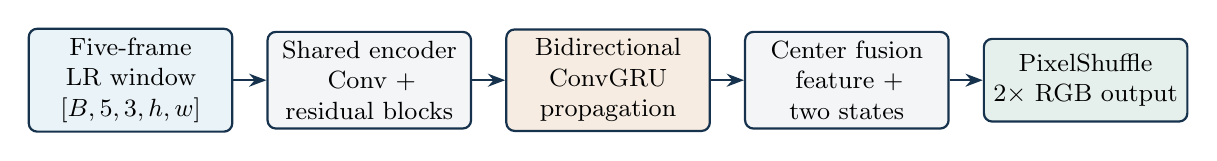
\begin{tikzpicture}[
  node distance=0.42cm,
  block/.style={
    rectangle,
    rounded corners=3pt,
    draw=navy,
    line width=0.8pt,
    align=center,
    minimum height=1.05cm,
    text width=2.35cm,
    font=\small
  },
  input/.style={block,fill=lightblue},
  process/.style={block,fill=lightgray},
  recurrent/.style={block,fill=orange!12},
  output/.style={block,fill=green!12},
  arrow/.style={-{Stealth[length=2.2mm]},line width=0.8pt,draw=navy}
]
\node[input] (window) {Five-frame LR window\\$[B,5,3,h,w]$};
\node[process,right=of window] (features) {Shared encoder\\Conv + residual blocks};
\node[recurrent,right=of features] (propagation) {Bidirectional\\ConvGRU propagation};
\node[process,right=of propagation] (fusion) {Center fusion\\feature + two states};
\node[output,right=of fusion] (upsample) {PixelShuffle\\$2\times$ RGB output};
\draw[arrow] (window) -- (features);
\draw[arrow] (features) -- (propagation);
\draw[arrow] (propagation) -- (fusion);
\draw[arrow] (fusion) -- (upsample);
\end{tikzpicture}
\caption{The \code{BasicVSRMini} inference path. Temporal information is
propagated in both directions and fused only at the center frame.}
\label{fig:model}
\end{figure}

\subsection*{Feature extraction and propagation}

Each LR frame is encoded independently by a shared convolutional feature
extractor:
\begin{equation}
  \mathbf{e}_t = E(\mathbf{x}_t).
\end{equation}
Forward and backward ConvGRU cells then aggregate temporal context:
\begin{align}
  \mathbf{h}^{\rightarrow}_t &=
    G_f(\mathbf{e}_t,\mathbf{h}^{\rightarrow}_{t-1}),\\
  \mathbf{h}^{\leftarrow}_t &=
    G_b(\mathbf{e}_t,\mathbf{h}^{\leftarrow}_{t+1}).
\end{align}
At center index $c$, the model concatenates
$[\mathbf{e}_c,\mathbf{h}^{\rightarrow}_c,\mathbf{h}^{\leftarrow}_c]$,
reduces the channels with a $1\times1$ convolution, applies residual
refinement, and reconstructs RGB with convolution plus PixelShuffle
\cite{shi2016pixelshuffle}.

This design borrows the bidirectional propagation principle of BasicVSR
\cite{chan2021basicvsr}, but omits its explicit optical-flow alignment and
sequence-wide reconstruction. The omission keeps the model compact and easy
to train, but limits robustness under large displacement, occlusion, and
scene changes.

\subsection*{Training objective}

The reported model uses an $L_1$ center-frame reconstruction loss:
\begin{equation}
  \mathcal{L}_1(\theta)=
  \frac{1}{|\Omega|}
  \sum_{u\in\Omega}
  \left|
    f_\theta(\mathbf{x}_{c-2:c+2})_u-\mathbf{y}_{c,u}
  \right|.
\end{equation}
Training uses Adam with learning rate $2\times10^{-4}$, batch size 4,
48 base channels, and 6 reconstruction residual blocks. The final run
continued to 150,000 steps; the best validation checkpoint occurred at
80,000 steps.

\reportsection{Data and Evaluation Protocol}

\subsection*{Data}

Training uses a union of Vimeo-90K-style sequence data. The checked-in local
evaluation set contains Vimeo-derived sequences arranged in a REDS-style
HR/LR directory structure. Sequence-level manifests avoid mixing neighboring
frames across scenes. During training, the loader selects aligned temporal
windows, applies scale-aligned crops and flips, and returns the HR center
frame as the target.

\callout{Benchmark caveat.}{
The validation IDs and folder layout resemble REDS, but the content is
Vimeo-derived. The reported values are valid for reproducing this repository's
pipeline and demo; they must not be presented as official REDS benchmark
results.
}

\subsection*{Image metrics}

Predictions are clamped to $[0,1]$ and cropped by two pixels on every border.
The primary domain is the BT.601-style Y channel. PSNR and SSIM are computed
per frame and averaged across the validation samples \cite{wang2004ssim}.

\subsection*{Temporal metrics}

The report includes two output-only temporal diagnostics:
\begin{itemize}
  \item \textbf{Difference energy}: mean absolute change between adjacent output frames. Lower is not automatically better because true scene motion also contributes.
  \item \textbf{tPSNR}: PSNR between adjacent outputs after Farneb\"ack optical-flow warping \cite{farneback2003}. Higher generally indicates smoother motion-compensated evolution, but the score inherits optical-flow errors.
\end{itemize}

Target-relative auditing is also implemented. The final temporal model has
temporal error energy 0.0105, compared with 0.0108 for bicubic and 0.0145 for
the undertrained single-frame checkpoint. These diagnostics are more
interpretable than raw smoothness alone because they compare predicted motion
with target motion.

\reportsection{Results}

\begin{table}[ht]
\centering
\caption{Local Vimeo-derived REDS-style evaluation. The single-frame model is
a 300-step pipeline baseline and is not budget matched.}
\label{tab:results}
\small
\begin{tabularx}{\linewidth}{
  >{\raggedright\arraybackslash}X
  r r r r r
}
\toprule
\textbf{Method} &
\textbf{PSNR-Y} &
\textbf{SSIM-Y} &
\textbf{tPSNR} &
\textbf{Diff.} &
\textbf{CPU ms/frame} \\
\midrule
Bicubic &
36.8033 & 0.9601 & 36.3441 & 0.0217 & 0.238 \\
Single-frame SR, 300 steps &
32.3755 & 0.8807 & 33.8817 & 0.0183 & 9.105 \\
\textbf{Temporal SR, 5 frames} &
\textbf{38.3265} & \textbf{0.9604} & \textbf{36.6018} &
\textbf{0.0201} & 34.941 \\
\bottomrule
\end{tabularx}
\end{table}

\callout{Primary finding.}{
The final temporal model improves PSNR-Y by \metric{+1.5231 dB} and tPSNR by
\metric{+0.2578 dB} over bicubic on the locked local evaluation set. It also
reduces raw difference energy from 0.0217 to 0.0201.
}

\begin{figure}[ht]
\centering
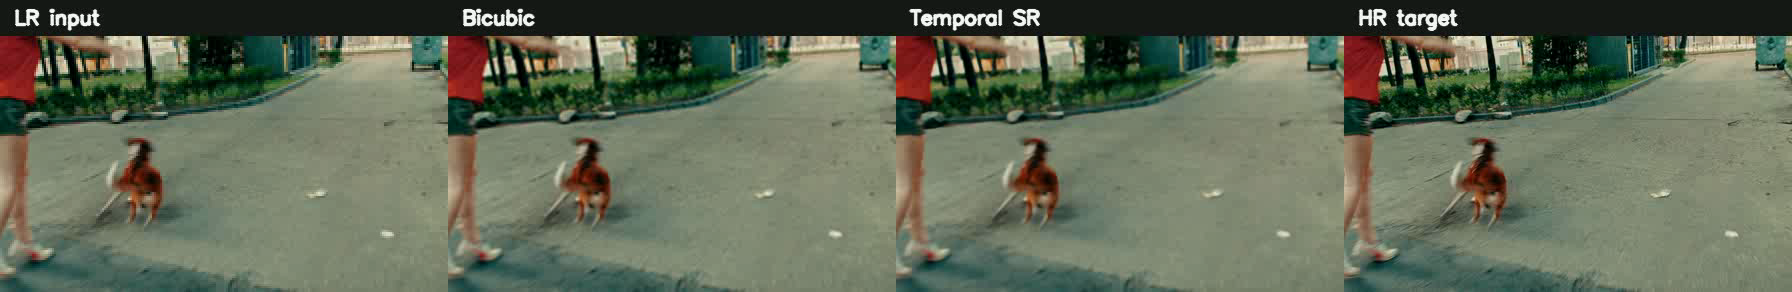
\includegraphics[
  width=\linewidth
]{../results/final/videos/final_temporal_vsr_5f_small_2x/all_val_comparison_preview.png}
\caption{Representative comparison generated by the final checkpoint. From
left to right: nearest-neighbor LR visualization, bicubic, temporal SR, and HR
target. The temporal output restores sharper structure than bicubic while
remaining visually close to the target.}
\label{fig:qualitative}
\end{figure}

\subsection*{Interpretation}

The PSNR result demonstrates that the temporal model learns useful information
beyond deterministic interpolation on this data distribution. The final model
also improves flow-warped tPSNR relative to bicubic, while its target-relative
temporal error is slightly lower. Together these results support the claim
that neighboring frames contribute both reconstruction quality and temporal
consistency.

The single-frame row should not be used to quantify the value of temporal
modeling. That checkpoint was trained for only 300 steps, whereas the final
temporal model was selected from a long run. Its lower raw difference energy
mainly reflects smoother, underfit outputs. A fair ablation requires matched
data, optimizer, parameter count, training steps, and checkpoint selection.

\reportsection{Deployment and Reproducibility}

\begin{table}[ht]
\centering
\caption{Final deployment artifacts and measured CPU latency.}
\small
\begin{tabularx}{\linewidth}{>{\bfseries\color{navy}}l X r}
\toprule
Artifact & Configuration & Result \\
\midrule
PyTorch demo & 240 frames, $64\times64$ LR, five-frame windows & 34.941 ms/frame \\
ONNX Runtime & CPUExecutionProvider, same clip, 10 warmups & 21.589 ms/frame \\
ONNX graph & Dynamic batch and spatial axes; fixed temporal length & Export successful \\
\bottomrule
\end{tabularx}
\end{table}

The ONNX Runtime measurement is 38.2\% lower latency than the PyTorch CPU
demo on the same clip. This is a deployment comparison, not a hardware-neutral
real-time claim. The current sliding-window path recomputes overlapping
features and recurrent states for every output frame, leaving substantial room
for streaming-state reuse.

The repository preserves the full training configuration in checkpoints and
stores training and validation metrics as JSONL. The key reproducibility
artifacts are:
\begin{itemize}
  \item \code{configs/temporal\_small.toml};
  \item \code{results/runs/temporal\_vsr\_5f\_small\_2x/checkpoints/best.pt};
  \item \code{results/final/tables/final\_comparison.md};
  \item \code{results/onnx/temporal\_vsr\_5f\_small\_2x.onnx};
  \item final comparison images and videos under \code{results/final/videos/}.
\end{itemize}

\reportsection{Limitations and Next Steps}

\begin{enumerate}
  \item \textbf{Evaluation validity.} Rerun the locked protocol on official REDS data before making benchmark claims.
  \item \textbf{Fair baseline.} Train a budget-matched single-frame model before attributing gains specifically to temporal context.
  \item \textbf{Motion handling.} Add flow-guided or deformable alignment for large motion, occlusion, and fine repeated textures.
  \item \textbf{Temporal objective.} Evaluate target-relative consistency or warping losses instead of relying only on center-frame $L_1$.
  \item \textbf{Runtime.} Cache frame features and recurrent state across overlapping windows; then benchmark GPU, FP16, and quantized inference.
  \item \textbf{Testing.} Add automated coverage for window indexing, metric formulas, checkpoint resume, ONNX parity, and boundary-frame padding.
\end{enumerate}

\newpage
\reportsection{Conclusion}

\project{} is a credible compact implementation of temporal video
super-resolution. Its main contribution is not a claim of DLSS equivalence;
it is a readable, reproducible path from temporal-window data loading through
training, evaluation, qualitative evidence, and ONNX deployment. The final
checkpoint clearly outperforms bicubic on the locked local validation set,
while the report's caveats identify exactly what remains necessary for a fair
research comparison and broader deployment claim.

\begin{thebibliography}{9}
\small

\bibitem{chan2021basicvsr}
K. C. K. Chan, X. Wang, K. Yu, C. Dong, and C. C. Loy,
``BasicVSR: The Search for Essential Components in Video
Super-Resolution and Beyond,'' in \emph{CVPR}, 2021.

\bibitem{chan2022basicvsrpp}
K. C. K. Chan, S. Zhou, X. Xu, and C. C. Loy,
``BasicVSR++: Improving Video Super-Resolution with Enhanced Propagation
and Alignment,'' in \emph{CVPR Workshops}, 2022.

\bibitem{wang2019edvr}
X. Wang, K. C. K. Chan, K. Yu, C. Dong, and C. C. Loy,
``EDVR: Video Restoration with Enhanced Deformable Convolutional
Networks,'' in \emph{CVPR Workshops}, 2019.

\bibitem{shi2016pixelshuffle}
W. Shi et al.,
``Real-Time Single Image and Video Super-Resolution Using an Efficient
Sub-Pixel Convolutional Neural Network,'' in \emph{CVPR}, 2016.

\bibitem{xue2019toflow}
T. Xue, B. Chen, J. Wu, D. Wei, and W. T. Freeman,
``Video Enhancement with Task-Oriented Flow,''
\emph{International Journal of Computer Vision}, vol. 127, no. 8, 2019.

\bibitem{wang2004ssim}
Z. Wang, A. C. Bovik, H. R. Sheikh, and E. P. Simoncelli,
``Image Quality Assessment: From Error Visibility to Structural
Similarity,'' \emph{IEEE Transactions on Image Processing}, vol. 13,
no. 4, 2004.

\bibitem{farneback2003}
G. Farneb\"ack,
``Two-Frame Motion Estimation Based on Polynomial Expansion,'' in
\emph{Image Analysis}, 2003.

\bibitem{kingma2015adam}
D. P. Kingma and J. Ba,
``Adam: A Method for Stochastic Optimization,'' in \emph{ICLR}, 2015.

\end{thebibliography}

\end{document}
